\documentclass[11pt,a4paper]{article}

\usepackage[T1]{fontenc}
\usepackage[utf8]{inputenc}
\usepackage[french]{babel}
\usepackage{geometry}
\usepackage{graphicx}
\usepackage{hyperref}
\usepackage{caption}
\usepackage{enumitem}
\usepackage{booktabs}

\geometry{margin=2.5cm}
\hypersetup{colorlinks=true, linkcolor=blue, urlcolor=blue}

\title{Compte rendu --- Atelier DevOps CI/CD\\Projet \texttt{calculatrice-cicd}}
\author{Younes BASIR \\ UPF --- DevOps}
\date{\today}

\begin{document}

\maketitle

\section{Introduction}

Dans le cadre de l'atelier DevOps, j'ai mis en place une chaîne \emph{CI/CD} (intégration et déploiement continus) pour une petite application Python nommée \texttt{calculatrice-cicd}. L'objectif était de vérifier automatiquement le code à chaque modification, puis de simuler un déploiement lorsque tout est correct.

J'ai utilisé \textbf{pytest} pour les tests, \textbf{flake8} pour le style et \textbf{GitHub Actions} pour la pipeline. Le dépôt est hébergé sur GitHub ; chaque \texttt{push} et chaque \texttt{pull request} vers la branche \texttt{main} déclenche les jobs définis dans \texttt{.github/workflows/pipeline.yml}.

\section{Notions CI/CD}

\textbf{Intégration continue (CI)} : à chaque modification envoyée sur le dépôt, le code est récupéré, analysé (lint) et testé automatiquement sur une machine neutre (runner).

\textbf{Livraison continue} : le code validé par la CI est toujours prêt à être mis en production ; la mise en ligne peut rester déclenchée manuellement.

\textbf{Déploiement continu} : si tous les contrôles passent, la mise en ligne (ici simulée) s'exécute sans intervention.

La pipeline construite suit le schéma suivant : les jobs \textbf{Lint} et \textbf{Test} s'exécutent en parallèle ; \textbf{Build} ne démarre que si les deux réussissent ; \textbf{Deploy} ne démarre que si \textbf{Build} réussit et uniquement sur la branche \texttt{main} (condition \texttt{if: github.ref == 'refs/heads/main'}).

\section{Étapes réalisées}

\subsection{Création du projet Python}

J'ai créé le projet avec les fichiers suivants :
\begin{itemize}[noitemsep]
  \item \texttt{calculatrice.py} : fonctions \texttt{addition}, \texttt{soustraction}, \texttt{multiplication} et \texttt{division} ;
  \item \texttt{test\_calculatrice.py} : cinq tests unitaires au départ, puis six après l'ajout de \texttt{puissance} ;
  \item \texttt{requirements.txt} : dépendance \texttt{pytest} ;
  \item \texttt{.gitignore} : exclusion de \texttt{venv/}, \texttt{\_\_pycache\_\_/} et \texttt{.pytest\_cache/}.
\end{itemize}

La division par zéro lève une \texttt{ValueError}, ce qui est testé avec \texttt{pytest.raises}.

\begin{figure}[htbp]
  \centering
  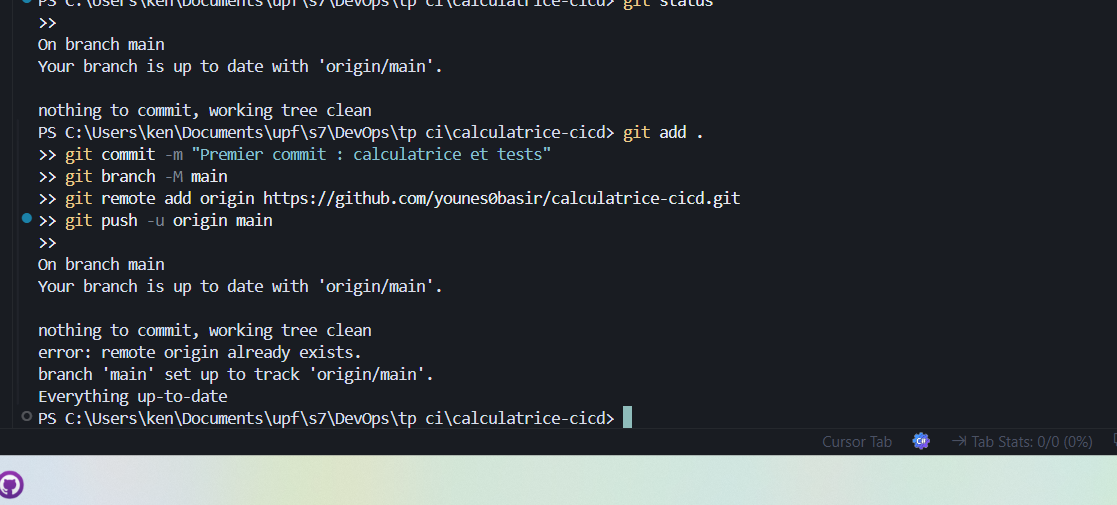
\includegraphics[width=0.92\textwidth]{git.png}
  \caption{Dépôt GitHub \texttt{calculatrice-cicd} avec les fichiers du premier commit.}
\end{figure}

\subsection{Tests et lint en local}

En local, j'ai installé les dépendances, lancé les tests puis vérifié le style comme le fera la pipeline :
\begin{verbatim}
python -m pip install -r requirements.txt
python -m pytest -v
python -m pip install flake8
python -m flake8 . --max-line-length=100
\end{verbatim}

Cinq tests sont passés et \texttt{flake8} n'a signalé aucune erreur avant le premier envoi sur GitHub.

\begin{figure}[htbp]
  \centering
  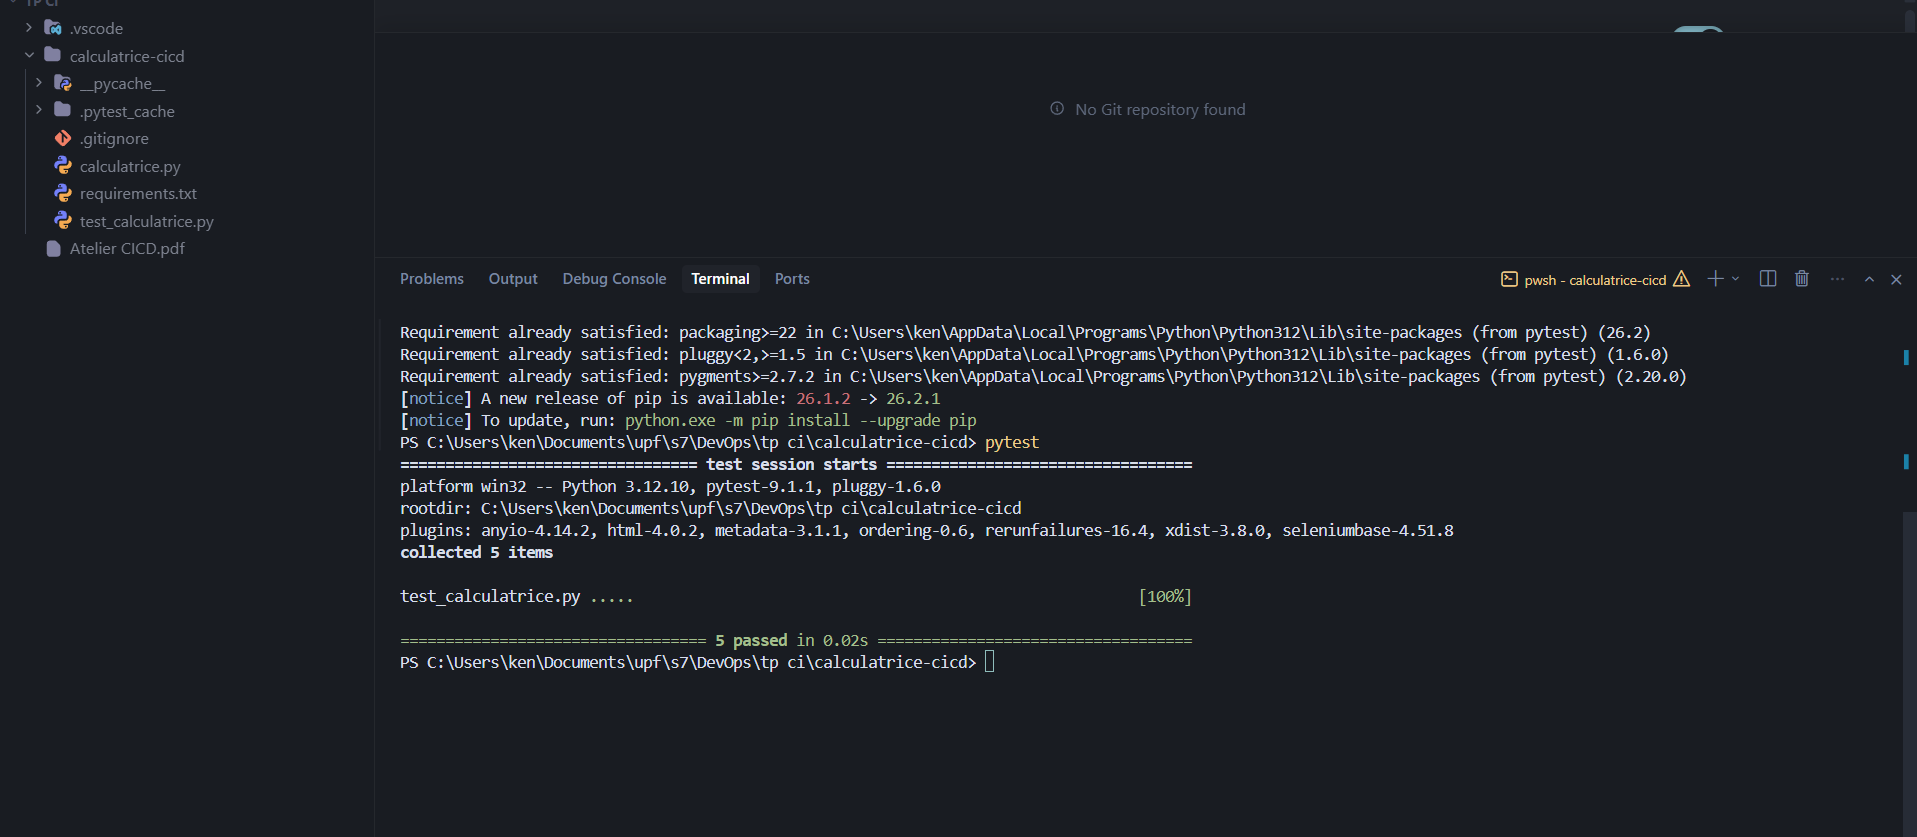
\includegraphics[width=0.92\textwidth]{pytest.png}
  \caption{Résultat de \texttt{pytest -v} en local (5 tests réussis).}
\end{figure}

\begin{figure}[htbp]
  \centering
  \includegraphics[width=0.92\textwidth]{flake8.png}
  \caption{Vérification du style avec \texttt{flake8} en local (aucune sortie = succès).}
\end{figure}

\subsection{Mise en place de GitHub Actions}

J'ai ajouté le fichier \texttt{.github/workflows/pipeline.yml} (nom affiché : \emph{Pipeline CI/CD Calculatrice}). La pipeline contient quatre jobs :
\begin{enumerate}[noitemsep]
  \item \textbf{Lint} : \texttt{flake8 . --max-line-length=100} sur Ubuntu, Python 3.12 ;
  \item \textbf{Test} : \texttt{pytest -v} après installation de \texttt{requirements.txt} ;
  \item \textbf{Build} : copie de \texttt{calculatrice.py} dans \texttt{dist/}, artefact \texttt{calculatrice-paquet} (\texttt{needs: [lint, test]}) ;
  \item \textbf{Deploy} : téléchargement de l'artefact, \texttt{ls -l dist/}, message simulé (\texttt{needs: build}, condition \texttt{main} uniquement).
\end{enumerate}

Les déclencheurs sont un \texttt{push} sur \texttt{main} et une \texttt{pull\_request} vers \texttt{main}.

\begin{figure}[htbp]
  \centering
  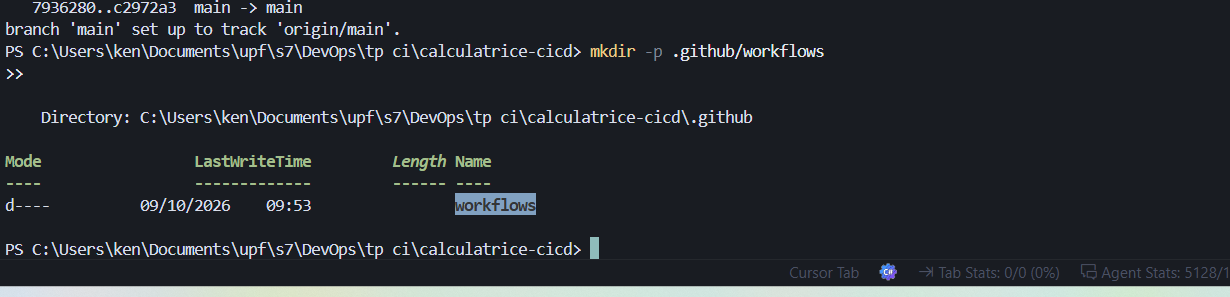
\includegraphics[width=0.92\textwidth]{workflow.png}
  \caption{Création du dossier \texttt{.github/workflows}.}
\end{figure}

\begin{figure}[htbp]
  \centering
  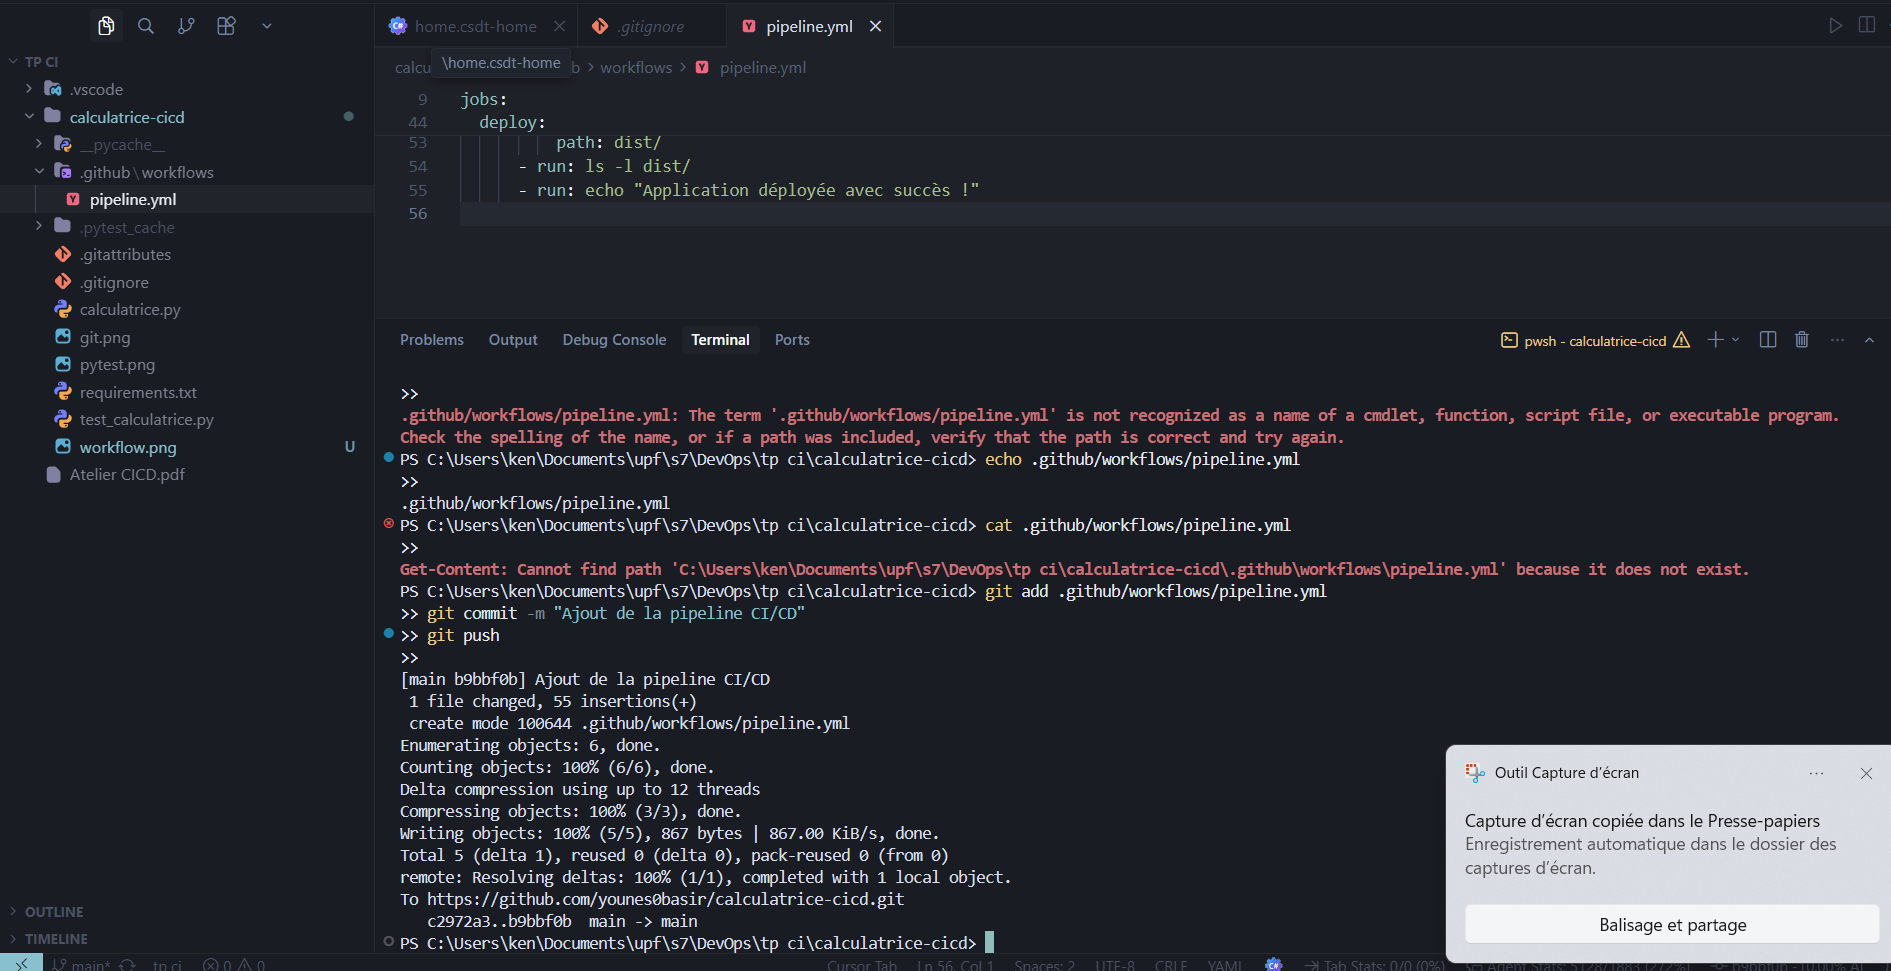
\includegraphics[width=0.92\textwidth]{PIPELINE.png}
  \caption{Fichier \texttt{pipeline.yml} et envoi du workflow sur GitHub.}
\end{figure}

\subsection{Observation de la pipeline (premier push réussi)}

Après le \texttt{push} du workflow, j'ai ouvert l'onglet \emph{Actions}, la dernière exécution, puis la page \emph{Summary}. Le graphique montre \textbf{Lint} et \textbf{Test} côte à côte, puis \textbf{Build}, puis \textbf{Deploy}. J'ai consulté les logs du job \emph{Tests automatiques} (les cinq tests visibles comme en local), téléchargé l'artefact \texttt{calculatrice-paquet} (archive contenant \texttt{calculatrice.py}) et lu le log du job \emph{Déploiement (simulé)}.

\begin{figure}[htbp]
  \centering
  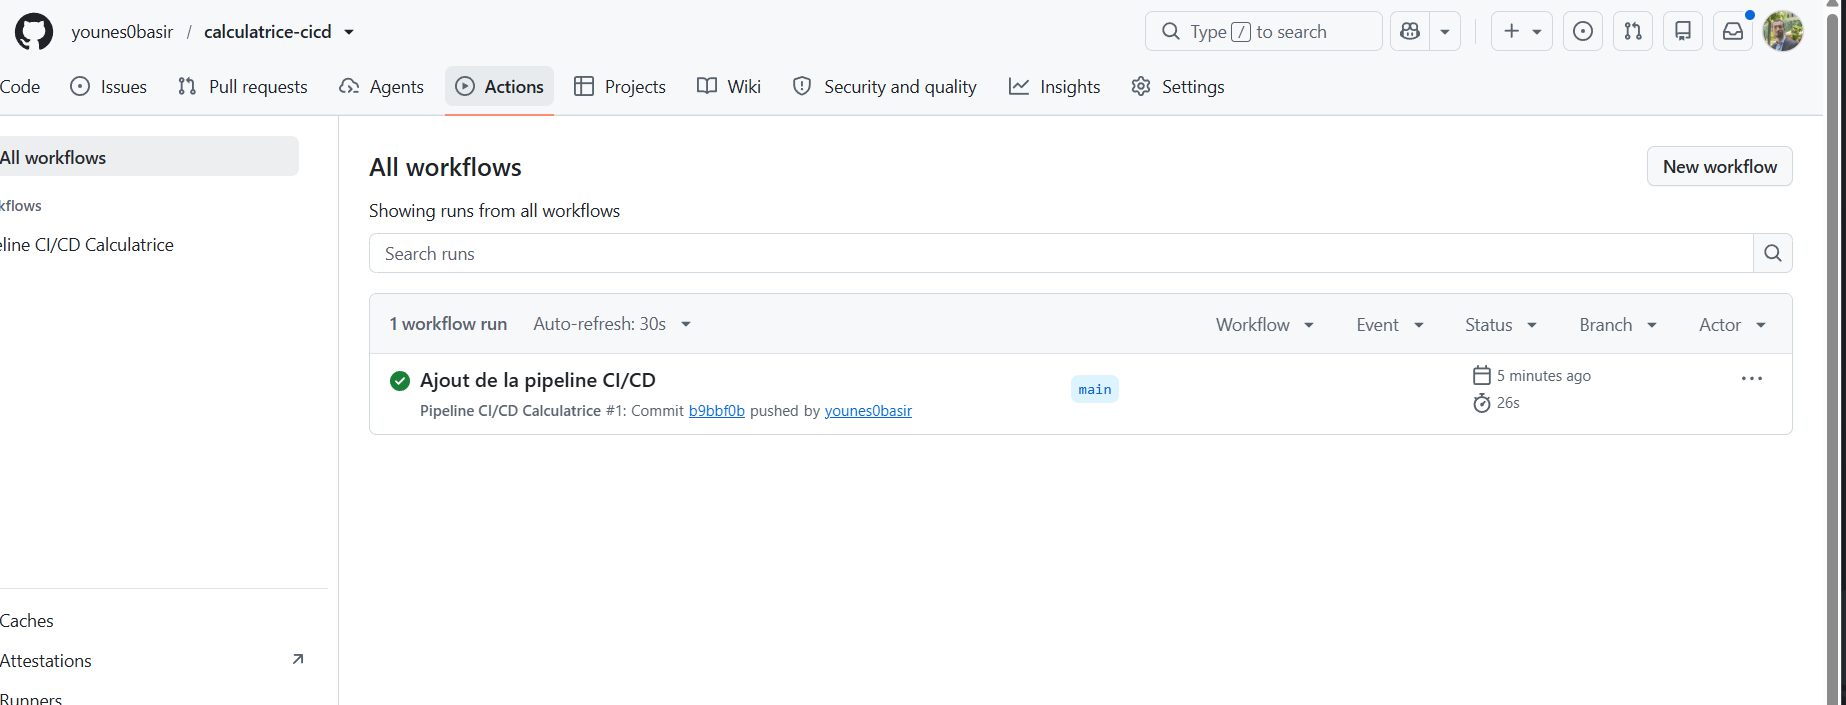
\includegraphics[width=0.92\textwidth]{github_actions.png}
  \caption{Liste des exécutions ou vue d'ensemble dans l'onglet Actions.}
\end{figure}

\begin{figure}[htbp]
  \centering
  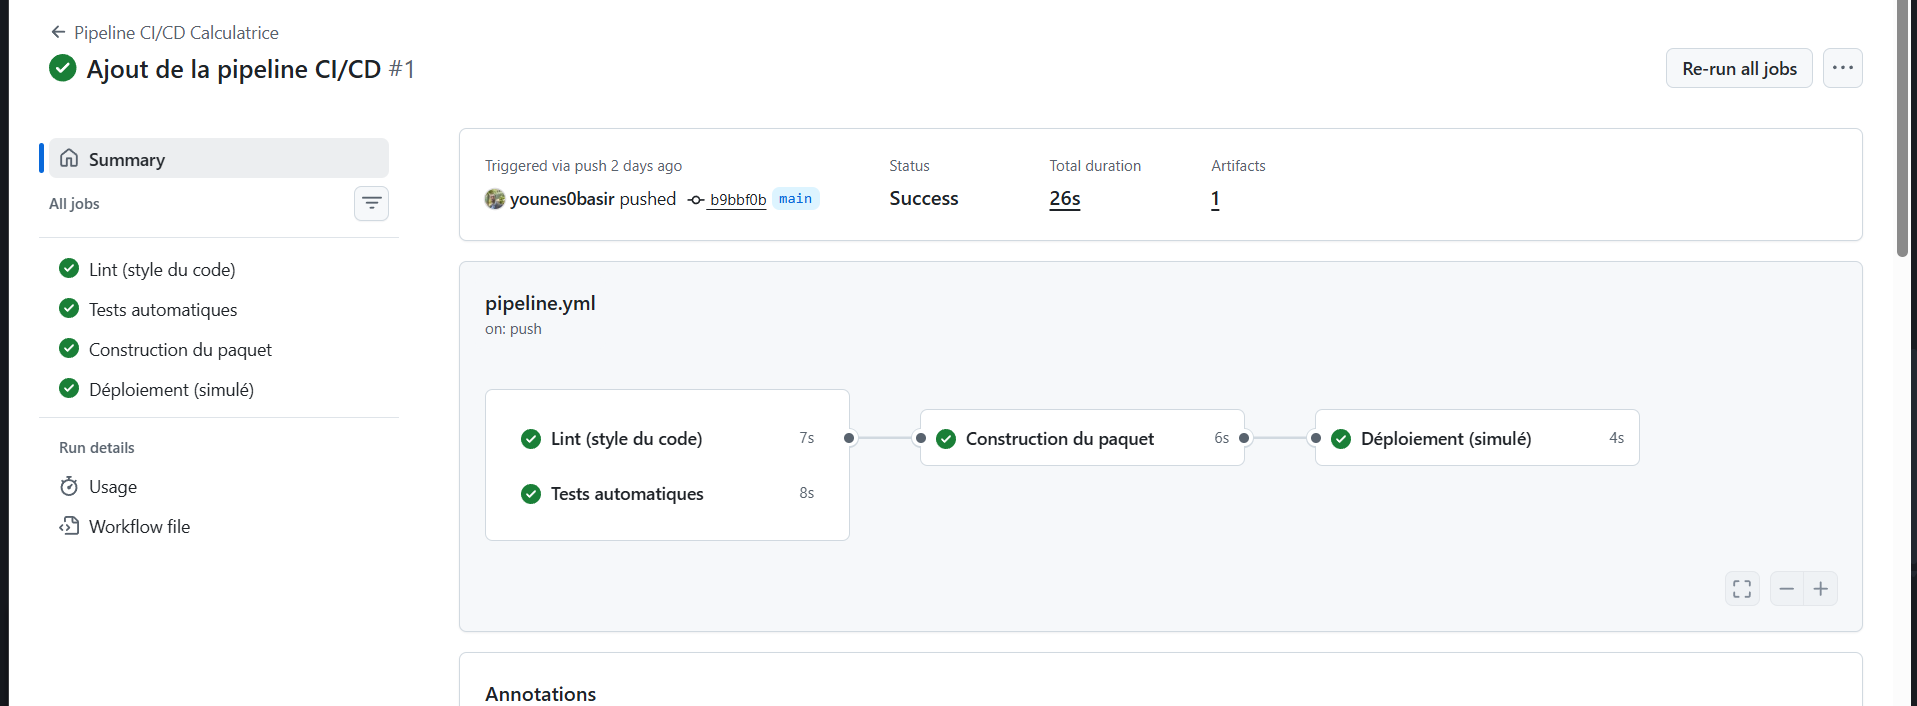
\includegraphics[width=0.92\textwidth]{pipeline-graph.png}
  \caption{Graphique des quatre jobs (Lint et Test en parallèle, puis Build et Deploy).}
\end{figure}

\begin{figure}[htbp]
  \centering
  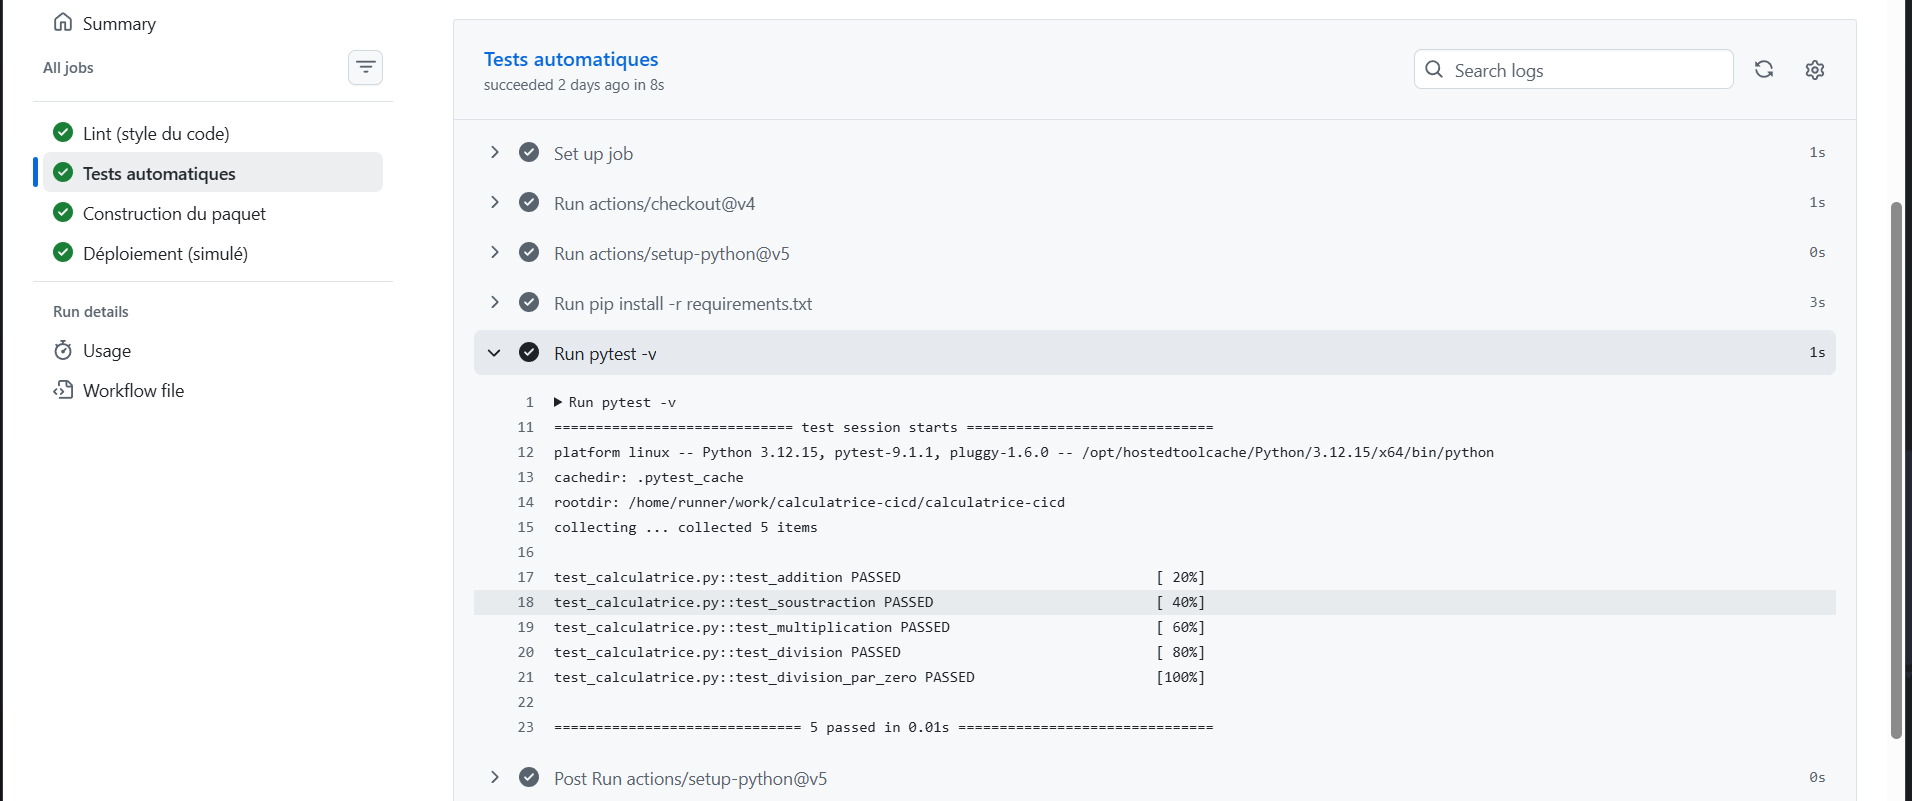
\includegraphics[width=0.92\textwidth]{pytest-actions-log.png}
  \caption{Logs du job \emph{Tests automatiques} (\texttt{pytest -v}).}
\end{figure}

\begin{figure}[htbp]
  \centering
  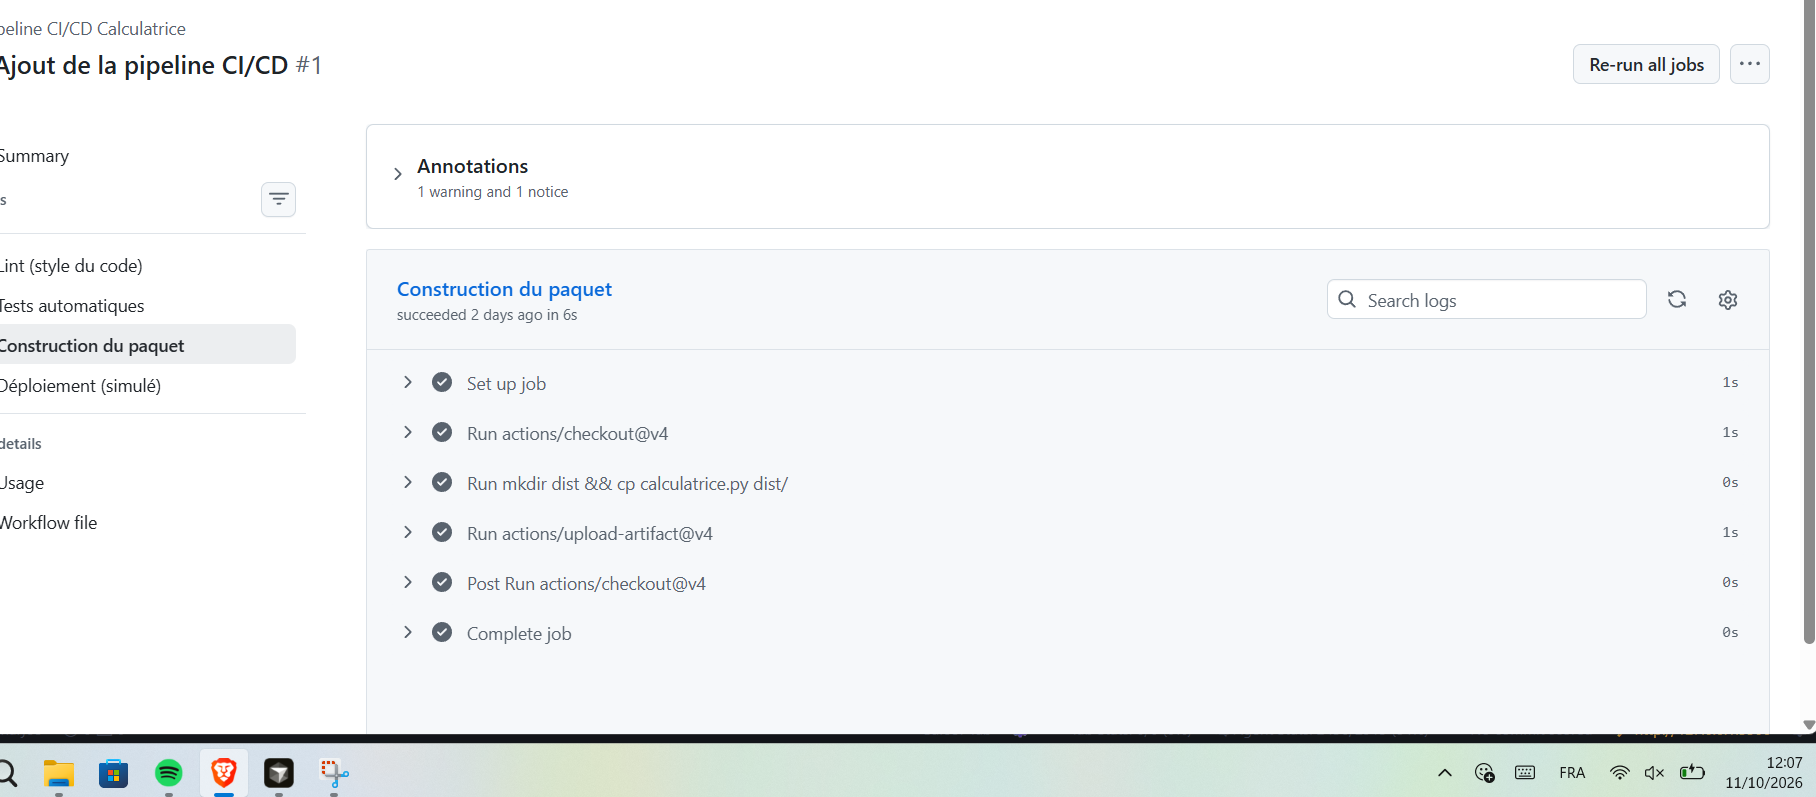
\includegraphics[width=0.92\textwidth]{artifact-calculatrice-paquet.png}
  \caption{Section \emph{Artifacts} : téléchargement de \texttt{calculatrice-paquet}.}
\end{figure}

\begin{figure}[htbp]
  \centering
  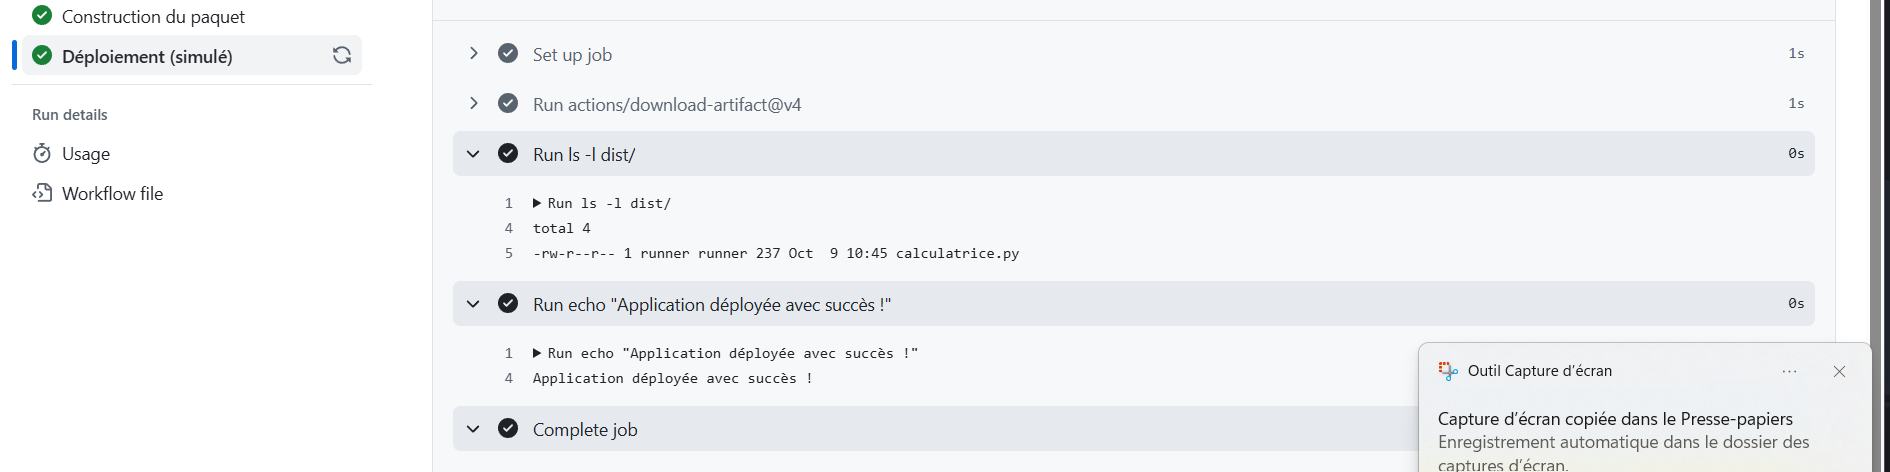
\includegraphics[width=0.92\textwidth]{deploy-log.png}
  \caption{Log du job \emph{Déploiement (simulé)} (message de succès simulé).}
\end{figure}

\subsection{Bug volontaire et correction (filet de sécurité)}

Pour vérifier que la pipeline bloque un code incorrect, j'ai modifié \texttt{addition} en remplaçant \texttt{a + b} par \texttt{a - b}. En local, \texttt{pytest -v} a échoué sur \texttt{test\_addition}. J'ai malgré tout poussé le commit (\emph{Bug volontaire dans l'addition}).

Sur GitHub Actions, le job \textbf{Test} est passé au rouge. Les jobs \textbf{Build} et \textbf{Deploy} ne se sont pas exécutés (état gris / ignoré) : le code défectueux n'a donc pas été « déployé ». Après remise de \texttt{a + b}, vérification locale (\texttt{5 passed}) et push de correction, une nouvelle exécution est repassée entièrement au vert.

\begin{figure}[htbp]
  \centering
  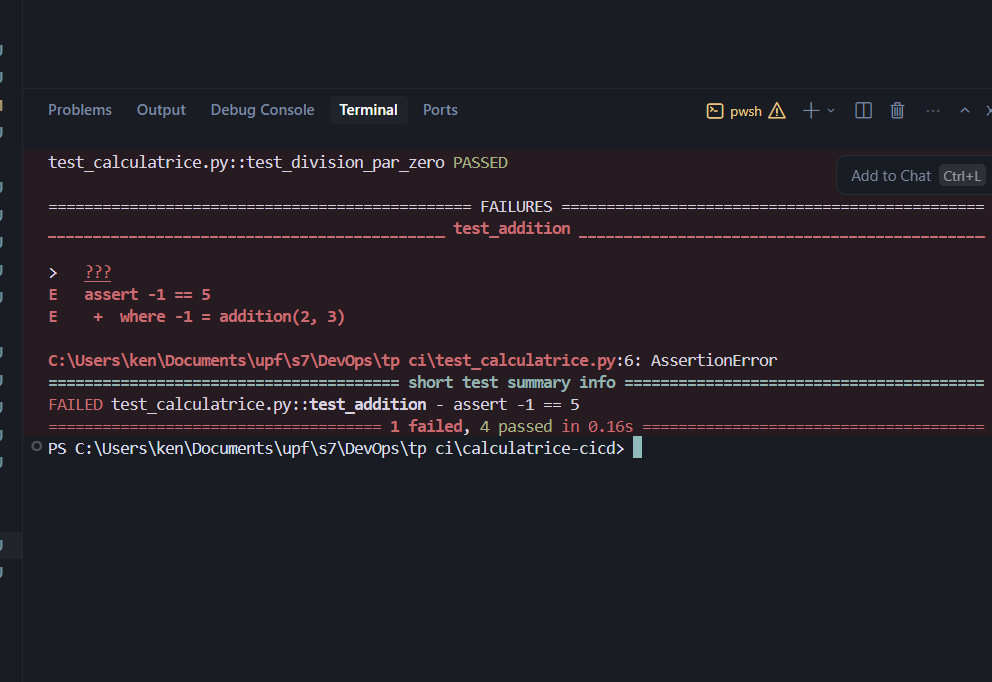
\includegraphics[width=0.92\textwidth]{pytest-bug-local.png}
  \caption{\texttt{pytest} en local après introduction du bug (échec de \texttt{test\_addition}).}
\end{figure}

\begin{figure}[htbp]
  \centering
  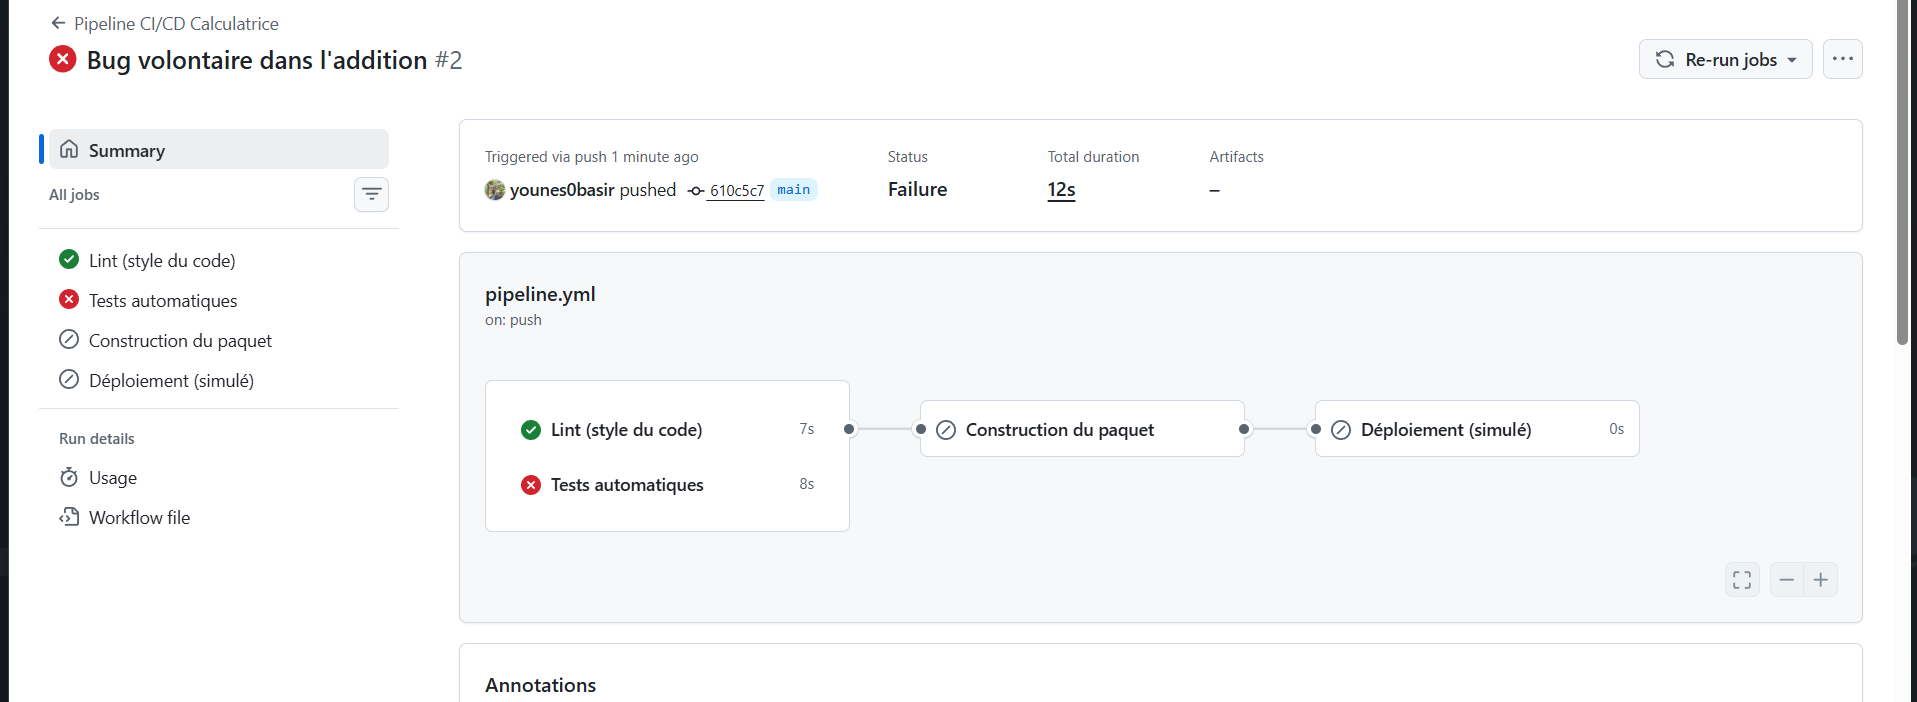
\includegraphics[width=0.92\textwidth]{pipeline-echec-test.png}
  \caption{Pipeline en échec : job \emph{Tests automatiques} rouge, Build et Deploy non lancés.}
\end{figure}

\begin{figure}[htbp]
  \centering
  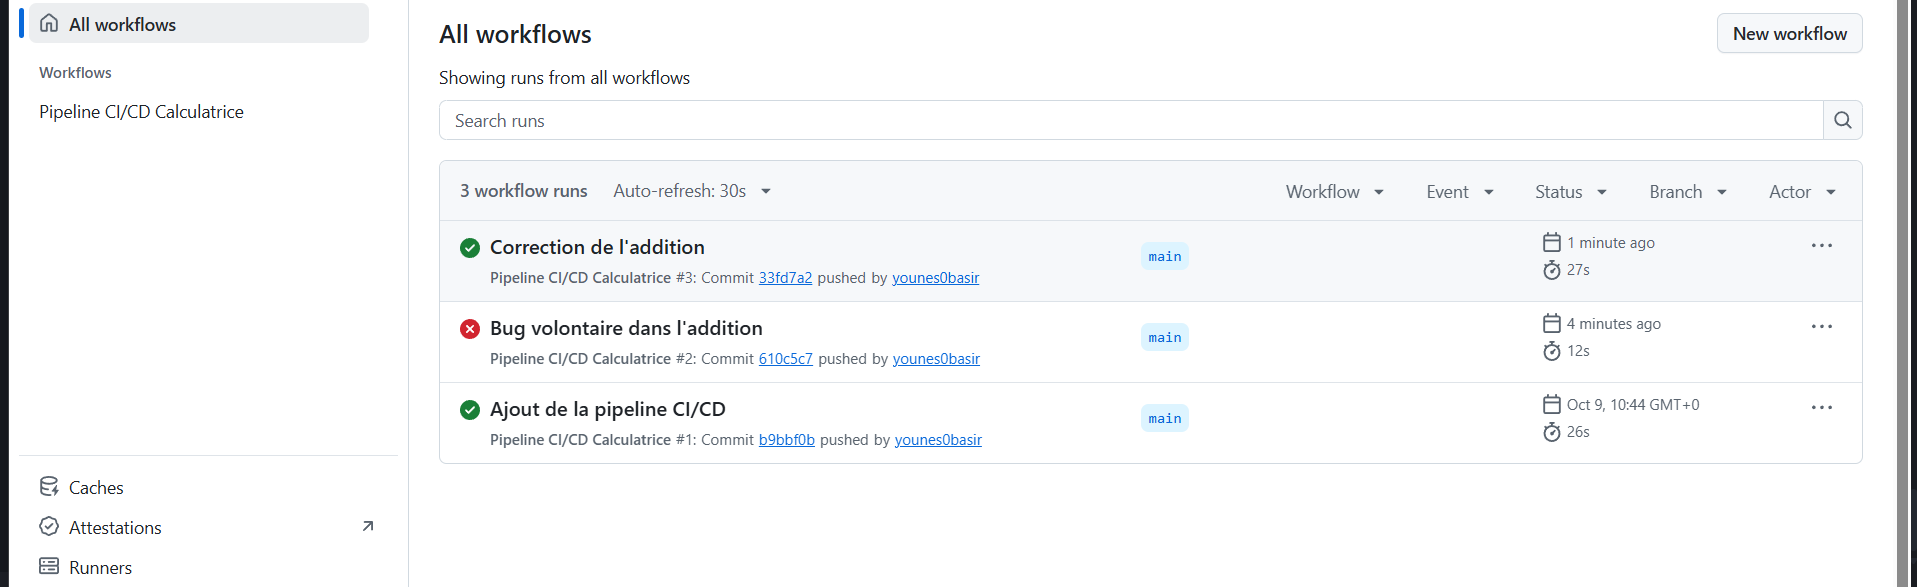
\includegraphics[width=0.92\textwidth]{pipeline-historique-rouge-vert.png}
  \caption{Historique Actions : une exécution rouge puis une exécution verte après correction.}
\end{figure}

\subsection{Branche \texttt{ajout-puissance} et Pull Request}

Pour simuler un flux d'équipe, j'ai créé la branche \texttt{ajout-puissance}, ajouté \texttt{puissance(a, b)} dans \texttt{calculatrice.py} et \texttt{test\_puissance} dans \texttt{test\_calculatrice.py}, puis poussé la branche. En local, \texttt{pytest -v} affichait \textbf{6 passed}.

J'ai ouvert une \textbf{Pull Request} vers \texttt{main}. La pipeline s'est exécutée sur la PR : \textbf{Lint}, \textbf{Test} et \textbf{Build} ont réussi, mais \textbf{Deploy} est resté \emph{skipped} (gris), car la condition \texttt{if} n'autorise le déploiement que depuis \texttt{main}, pas depuis une branche de PR.

Après \emph{Merge pull request}, une nouvelle exécution sur \texttt{main} a cette fois exécuté \textbf{Deploy} avec succès. La branche \texttt{main} contient alors la calculatrice complète, y compris \texttt{puissance}.

\begin{figure}[htbp]
  \centering
  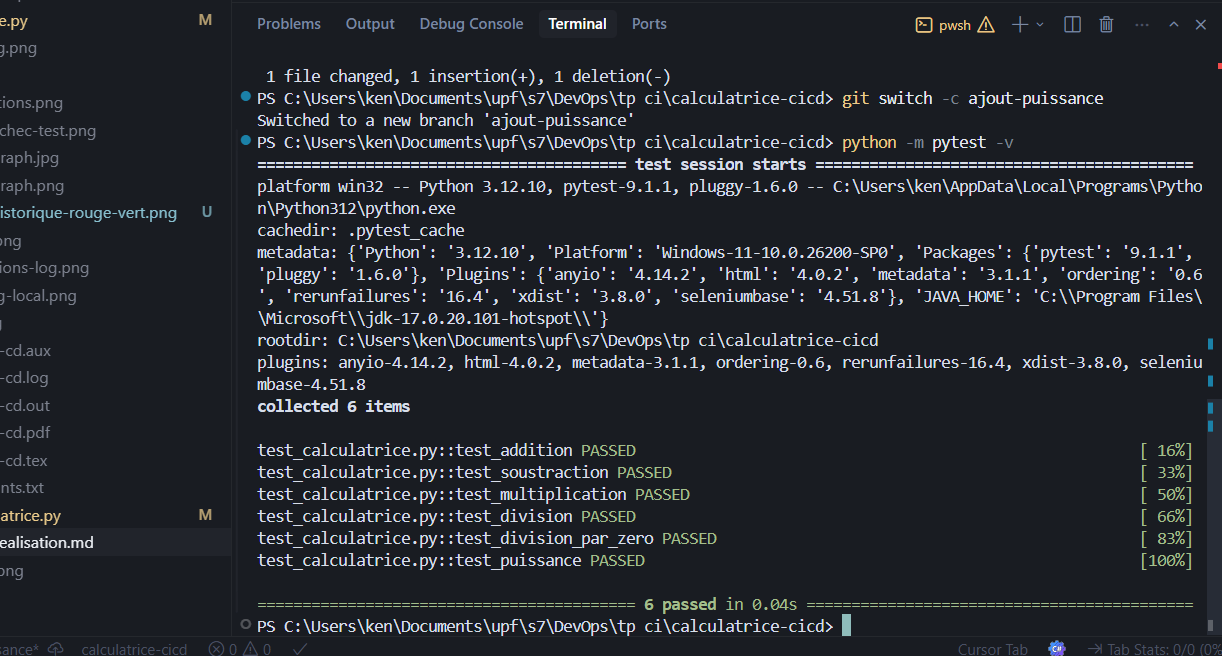
\includegraphics[width=0.92\textwidth]{pytest-6-tests.png}
  \caption{\texttt{pytest -v} en local après ajout de \texttt{puissance} (6 tests).}
\end{figure}

\begin{figure}[htbp]
  \centering
  \includegraphics[width=0.92\textwidth]{branche-ajout-puissance.png}
  \caption{Branche \texttt{ajout-puissance} sur GitHub (commits ou comparaison).}
\end{figure}

\begin{figure}[htbp]
  \centering
  \includegraphics[width=0.92\textwidth]{pr-checks-deploy-skipped.png}
  \caption{Pull Request : checks CI verts et job \emph{Deploy} ignoré (\emph{skipped}).}
\end{figure}

\begin{figure}[htbp]
  \centering
  \includegraphics[width=0.92\textwidth]{pipeline-main-deploy-vert.png}
  \caption{Pipeline sur \texttt{main} après fusion : les quatre jobs verts, Deploy inclus.}
\end{figure}

\section{Résultat final}

Le projet dispose d'une pipeline à quatre jobs, déclenchée automatiquement sur \texttt{push} et \texttt{pull\_request} vers \texttt{main}. Les tests et le lint garantissent la qualité ; un échec de test bloque build et déploiement. Le workflow branche $\rightarrow$ PR $\rightarrow$ merge $\rightarrow$ deploy sur \texttt{main} reproduit une pratique professionnelle de base. L'artefact \texttt{calculatrice-paquet} prouve que l'étape \textbf{Build} produit bien un livrable réutilisé par \textbf{Deploy}.

\section{Questions de réflexion}

\begin{enumerate}
  \item \textbf{CI vs déploiement continu :} la CI intègre et vérifie le code à chaque changement ; le déploiement continu publie automatiquement lorsque toutes les vérifications passent (ici le deploy est simulé et limité à \texttt{main}).
  \item \textbf{Deploy gris quand Test est rouge :} \textbf{Build} dépend de \textbf{Test} via \texttt{needs: [lint, test]} ; sans build réussi, \textbf{Deploy} ne démarre pas.
  \item \textbf{Lint et Test en parallèle :} les deux jobs sont indépendants ; les lancer ensemble réduit le temps total de la pipeline.
  \item \textbf{Sans \texttt{if} sur Deploy :} le déploiement simulé s'exécuterait aussi sur les branches de PR, ce qui n'est en général pas souhaitable.
  \item \textbf{Équipe de dix personnes :} même contrôle pour tous, traçabilité dans Actions, détection rapide des régressions, moins d'erreurs humaines ou de tests oubliés.
\end{enumerate}

\section{Conclusion}

Cet atelier m'a permis de comprendre l'intérêt du CI/CD : les tests et le lint ne dépendent plus d'une vérification manuelle à chaque changement. GitHub Actions automatise ce contrôle à chaque \texttt{push} et chaque PR. La simulation d'un bug puis sa correction montrent le rôle de filet de sécurité de la pipeline. Pour la suite, on pourrait ajouter un badge de statut, \texttt{pytest-cov}, une image Docker dans \textbf{Build} ou un déploiement réel (GitHub Pages, Render, etc.).

\end{document}
